%% 
%% Copyright 2007-2019 Elsevier Ltd
%% 
%% This file is part of the 'Elsarticle Bundle'.
%% ---------------------------------------------
%% 
%% It may be distributed under the conditions of the LaTeX Project Public
%% License, either version 1.2 of this license or (at your option) any
%% later version.  The latest version of this license is in
%%    http://www.latex-project.org/lppl.txt
%% and version 1.2 or later is part of all distributions of LaTeX
%% version 1999/12/01 or later.
%% 
%% The list of all files belonging to the 'Elsarticle Bundle' is
%% given in the file `manifest.txt'.
%% 
%% Template article for Elsevier's document class `elsarticle'
%% with harvard style bibliographic references

%%\documentclass[preprint,12pt,authoryear]{elsarticle}

%% Use the option review to obtain double line spacing
 \documentclass[authoryear,preprint,review,12pt]{elsarticle}

%% Use the options 1p,twocolumn; 3p; 3p,twocolumn; 5p; or 5p,twocolumn
%% for a journal layout:
%% \documentclass[final,1p,times,authoryear]{elsarticle}
%% \documentclass[final,1p,times,twocolumn,authoryear]{elsarticle}
%% \documentclass[final,3p,times,authoryear]{elsarticle}
%% \documentclass[final,3p,times,twocolumn,authoryear]{elsarticle}
%% \documentclass[final,5p,times,authoryear]{elsarticle}
%% \documentclass[final,5p,times,twocolumn,authoryear]{elsarticle}

%% For including figures, graphicx.sty has been loaded in
%% elsarticle.cls. If you prefer to use the old commands
%% please give \usepackage{epsfig}

%% The amssymb package provides various useful mathematical symbols
\usepackage{amssymb}
%% The amsthm package provides extended theorem environments
%% \usepackage{amsthm}

%% The lineno packages adds line numbers. Start line numbering with
%% \begin{linenumbers}, end it with \end{linenumbers}. Or switch it on
%% for the whole article with \linenumbers.
%% \usepackage{lineno}

\journal{Earth and Planetary Science Letters}

\begin{document}

\begin{frontmatter}

%% Title, authors and addresses

%% use the tnoteref command within \title for footnotes;
%% use the tnotetext command for theassociated footnote;
%% use the fnref command within \author or \address for footnotes;
%% use the fntext command for theassociated footnote;
%% use the corref command within \author for corresponding author footnotes;
%% use the cortext command for theassociated footnote;
%% use the ead command for the email address,
%% and the form \ead[url] for the home page:
%% \title{Title\tnoteref{label1}}
%% \tnotetext[label1]{}
%% \author{Name\corref{cor1}\fnref{label2}}
%% \ead{email address}
%% \ead[url]{home page}
%% \fntext[label2]{}
\cortext[cor1]{Corresponding author: paul.jarvis@unige.ch}
%% \address{Address\fnref{label3}}
%% \fntext[label3]{}

\title{Collective sedimentation from ash-clouds: insights from experimental buoyant, particle-laden gravity currents}

%% use optional labels to link authors explicitly to addresses:
%% \author[label1,label2]{}
%% \address[label1]{}
%% \address[label2]{}

\author[label1]{Paul A. Jarvis\corref{cor1}}
\author[label1]{Allan Fries}
\author[label1]{Jonathan Lemus}
\author[label1]{Costanza Bonadonna}
\author[label2]{Amanda Clarke}
\author[label3]{Irene Manzella}
\author[label4]{Jeremy Phillips}

\address[label1]{Department of Earth Sciences, University of Geneva, Rue des Mar{\"i}chers, Geneva, 1205, Switzerland}
\address[label2]{School of Earth and Space Exploration, Arizona State University, ISTB4-BLDG75, 781 E Terrance Mall, Tempe, AZ, 85287-6004, USA}
\address[label3]{School of Geography, Earth and Envrionmental Sciences, Univeristy of Plymouth, Drake Circus, Plymouth, PL4 8AA, UK}
\address[label4]{School of Earth Sciences, University of Bristol, Wills Memorial Building, Queens Road, Bristol, BS8 1RJ, UK}

\begin{abstract}
%% Text of abstract

\end{abstract}

%%Graphical abstract
\begin{graphicalabstract}
%\includegraphics{grabs}
\end{graphicalabstract}

%%Research highlights
\begin{highlights}
\item Research highlight 1
\item Research highlight 2
\end{highlights}

\begin{keyword}
%% keywords here, in the form: keyword \sep keyword

%% PACS codes here, in the form: \PACS code \sep code

%% MSC codes here, in the form: \MSC code \sep code
%% or \MSC[2008] code \sep code (2000 is the default)

\end{keyword}

\end{frontmatter}

%% \linenumbers

%% main text
\section{Introduction}
\label{sec:intro}

\section{Methods}
\label{sec:method}

Experiments were performed in a perspex flume of internal length 353 cm, width (12.2 $\pm$ 0.5) cm and depth 50 cm (Figure~\ref{fig:setup}). The uncertainty on the width is due to bowing of the tank walls. During the experimental setup, two removable gates can be placed at 24 and 53 cm, respectively, from the left-hand end, creating three sections. The left-most section takes no part in the experiment, whilst the short middle section is where the particle suspension is prepared, and is referred to as the gated section (length 27 cm). The remaining length of the flume is called the environment (length 3m).

\begin{figure}[ht!]
  \centerline{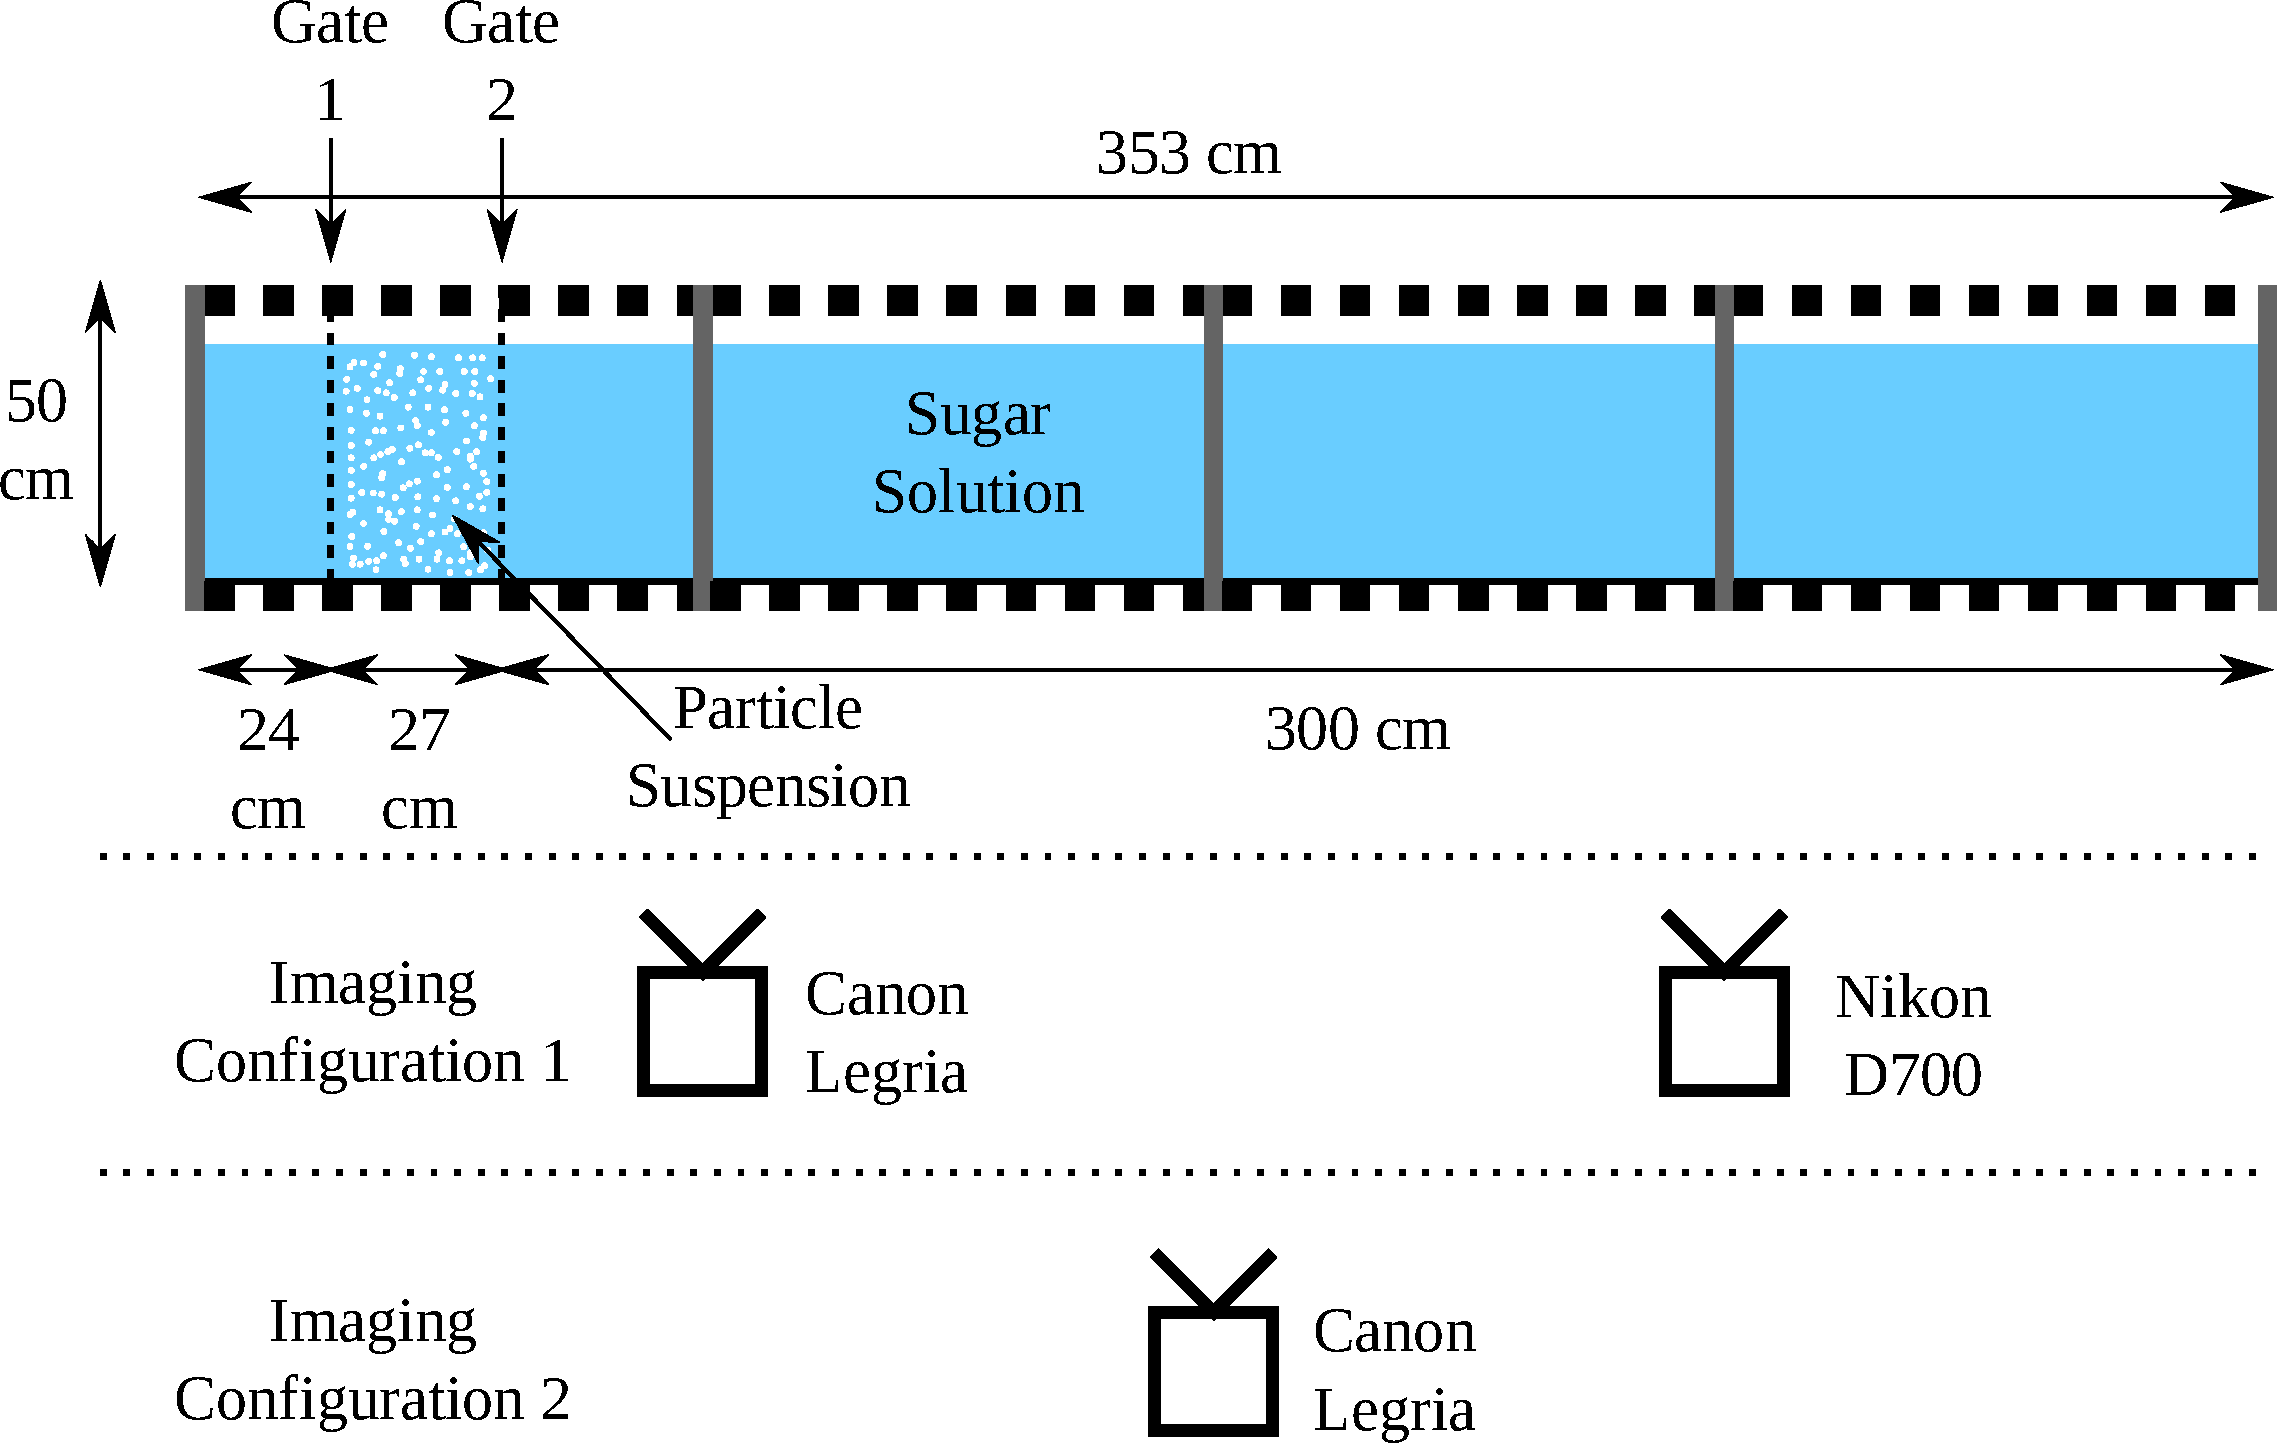
\includegraphics[width=0.9\textwidth]{setup.pdf}}
  \caption{Sketch showing the experimental setup. The flume is separated into three section separated by two gates. The leftmost section is not involved in the experiment. The rightmost section is a sugar solution of constant density whereas the section between gates 1 and 2 is a mixture of fresh water and ballotini. The concentration of particles is varied between experiments. The experiment is initiated by removing gate 2. Experiments were imaged using one of two configurations. }
  \label{fig:setup}
\end{figure}

The flume sits within a metal framework. Three vertical supports, each 3cm thick, at distances of 87 cm, 173.5 cm and 260 cm from the left-hand end prevent bowing. This effectively separates the flume into four, nearly equal, section. Behind each section a backing board is placed. For experiments with no particles, red or blue food colouring is added to the current and the backing board is white. Otherwise the boards are black. The top 5 cm of each board is a row of (5 $\times$ 5) cm$^{2}$ squares, alternating in colour from black-to-white. Meanwhile, at the base of the tank, tape is used to create a similar scale.

The day before an experiment, the flume is filled up to a depth of 47.5 cm. Separately, the desired mass of sugar is completely disolved in approximately 15 l of water. The flume and sugar solution are then both allowed to equilibrate to room temperature overnight. The next day, the flume is imaged (single frame) in its current configuration. In some experiments, the whole flume was imaged using a Canon Legria HFG40. In others, this camera was position closer to the tank, but only imaged the left-hand half of the flume, whilst the right-hand half was imaged using a Nikon D700 (DSLR). The captured frame(s) are used as reference images using the top(back) and bottom(front) scales. By capturing the image with the back scale partially submerged, it is possible to correct position measurements for distortion due to the refractive index (RI) of the water.

The flume water level is then lowered until it is of a depth of approximately 36.5 cm. Gates 1 and 2 are then put in place. The sugar solution is then added to the envrionment section. The gated section is then topped up with water until the water depth there is the same as the environment. This procedure results in a water depth of approximately 40 cm. The environment section is rigorously stirred. The RI of fluid from four positions in the environment section (top and bottom, near and far from the gate) is measured using a refractometer to ensure a uniform density. The RI of the gated section is also measured to check that there has been no significant leakage of sugar solution through the gate. A calibrated digital thermometer is used to measure the temperature of both sections. In all experiments, the maximum difference in temperature between the sections was 0.1 $^{\circ}$C.

Recording of the experiment then begins. The required mass of particles is added to the gated section which is thoroughly stirred to ensure a uniform particle concentration. Finally, gate 2 is removed and the particle suspension spreads along the free surface as a buoyant gravity current. Once the current head reaches the end of the tank, gate 2 is returned to its position and recording stops. 

The particles used were glass spheres with a density of (2.519 $\pm$ ??) g cm$^{-3}$, as measured by helium pycnometry using an Ultrapyc 1200e. They had a unimodal size distribution centred on a mode of 36 $\mu$m and a standard deviation of 12 $\mu$m, as determined from static light scattering using a Bettersizer S3 Plus. Figure~\ref{fig:size_dist} shows the measured size distribution of the particles. 

\begin{figure}[ht!]
  \centerline{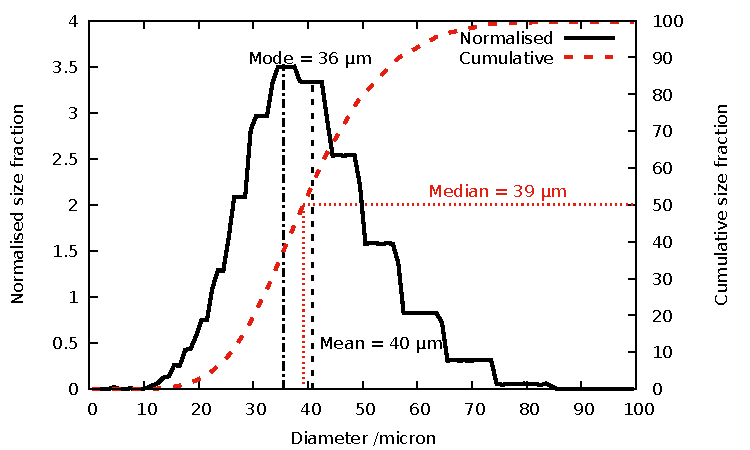
\includegraphics[width=0.9\textwidth]{unsieved_dist.pdf}}
  \caption{Normalised and cumulative volume-weighted size distributions of the particles used in the experiments.}
  \label{fig:size_dist}
\end{figure}

\section{Results}
\label{sec:res}

\subsection{Currents without particles}
\label{subsec:res_no_parts}

Figure~\ref{fig:GC3} shows the evolution of the current in experiment GC3.

\begin{figure}[ht!]
  \centerline{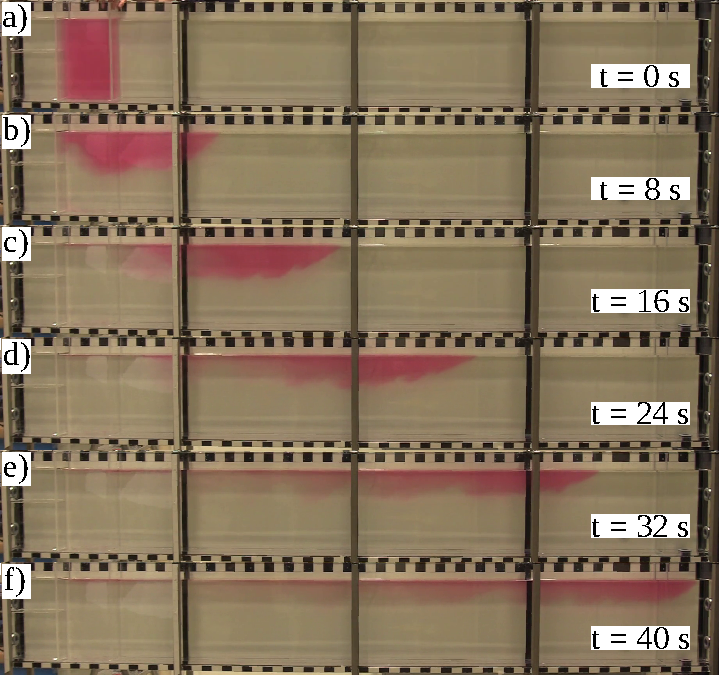
\includegraphics[width=0.9\textwidth]{GC3.pdf}}
  \caption{Sequence of images showing experiment GC3 ($\phi$ = 0, $g\prime$ = 0.162 m s$^{-2}$). }
  \label{fig:GC3}
\end{figure}

Figure~\ref{fig:GC9} shows the evolution of the current in experiment GC9.

\begin{figure}[ht!]
  \centerline{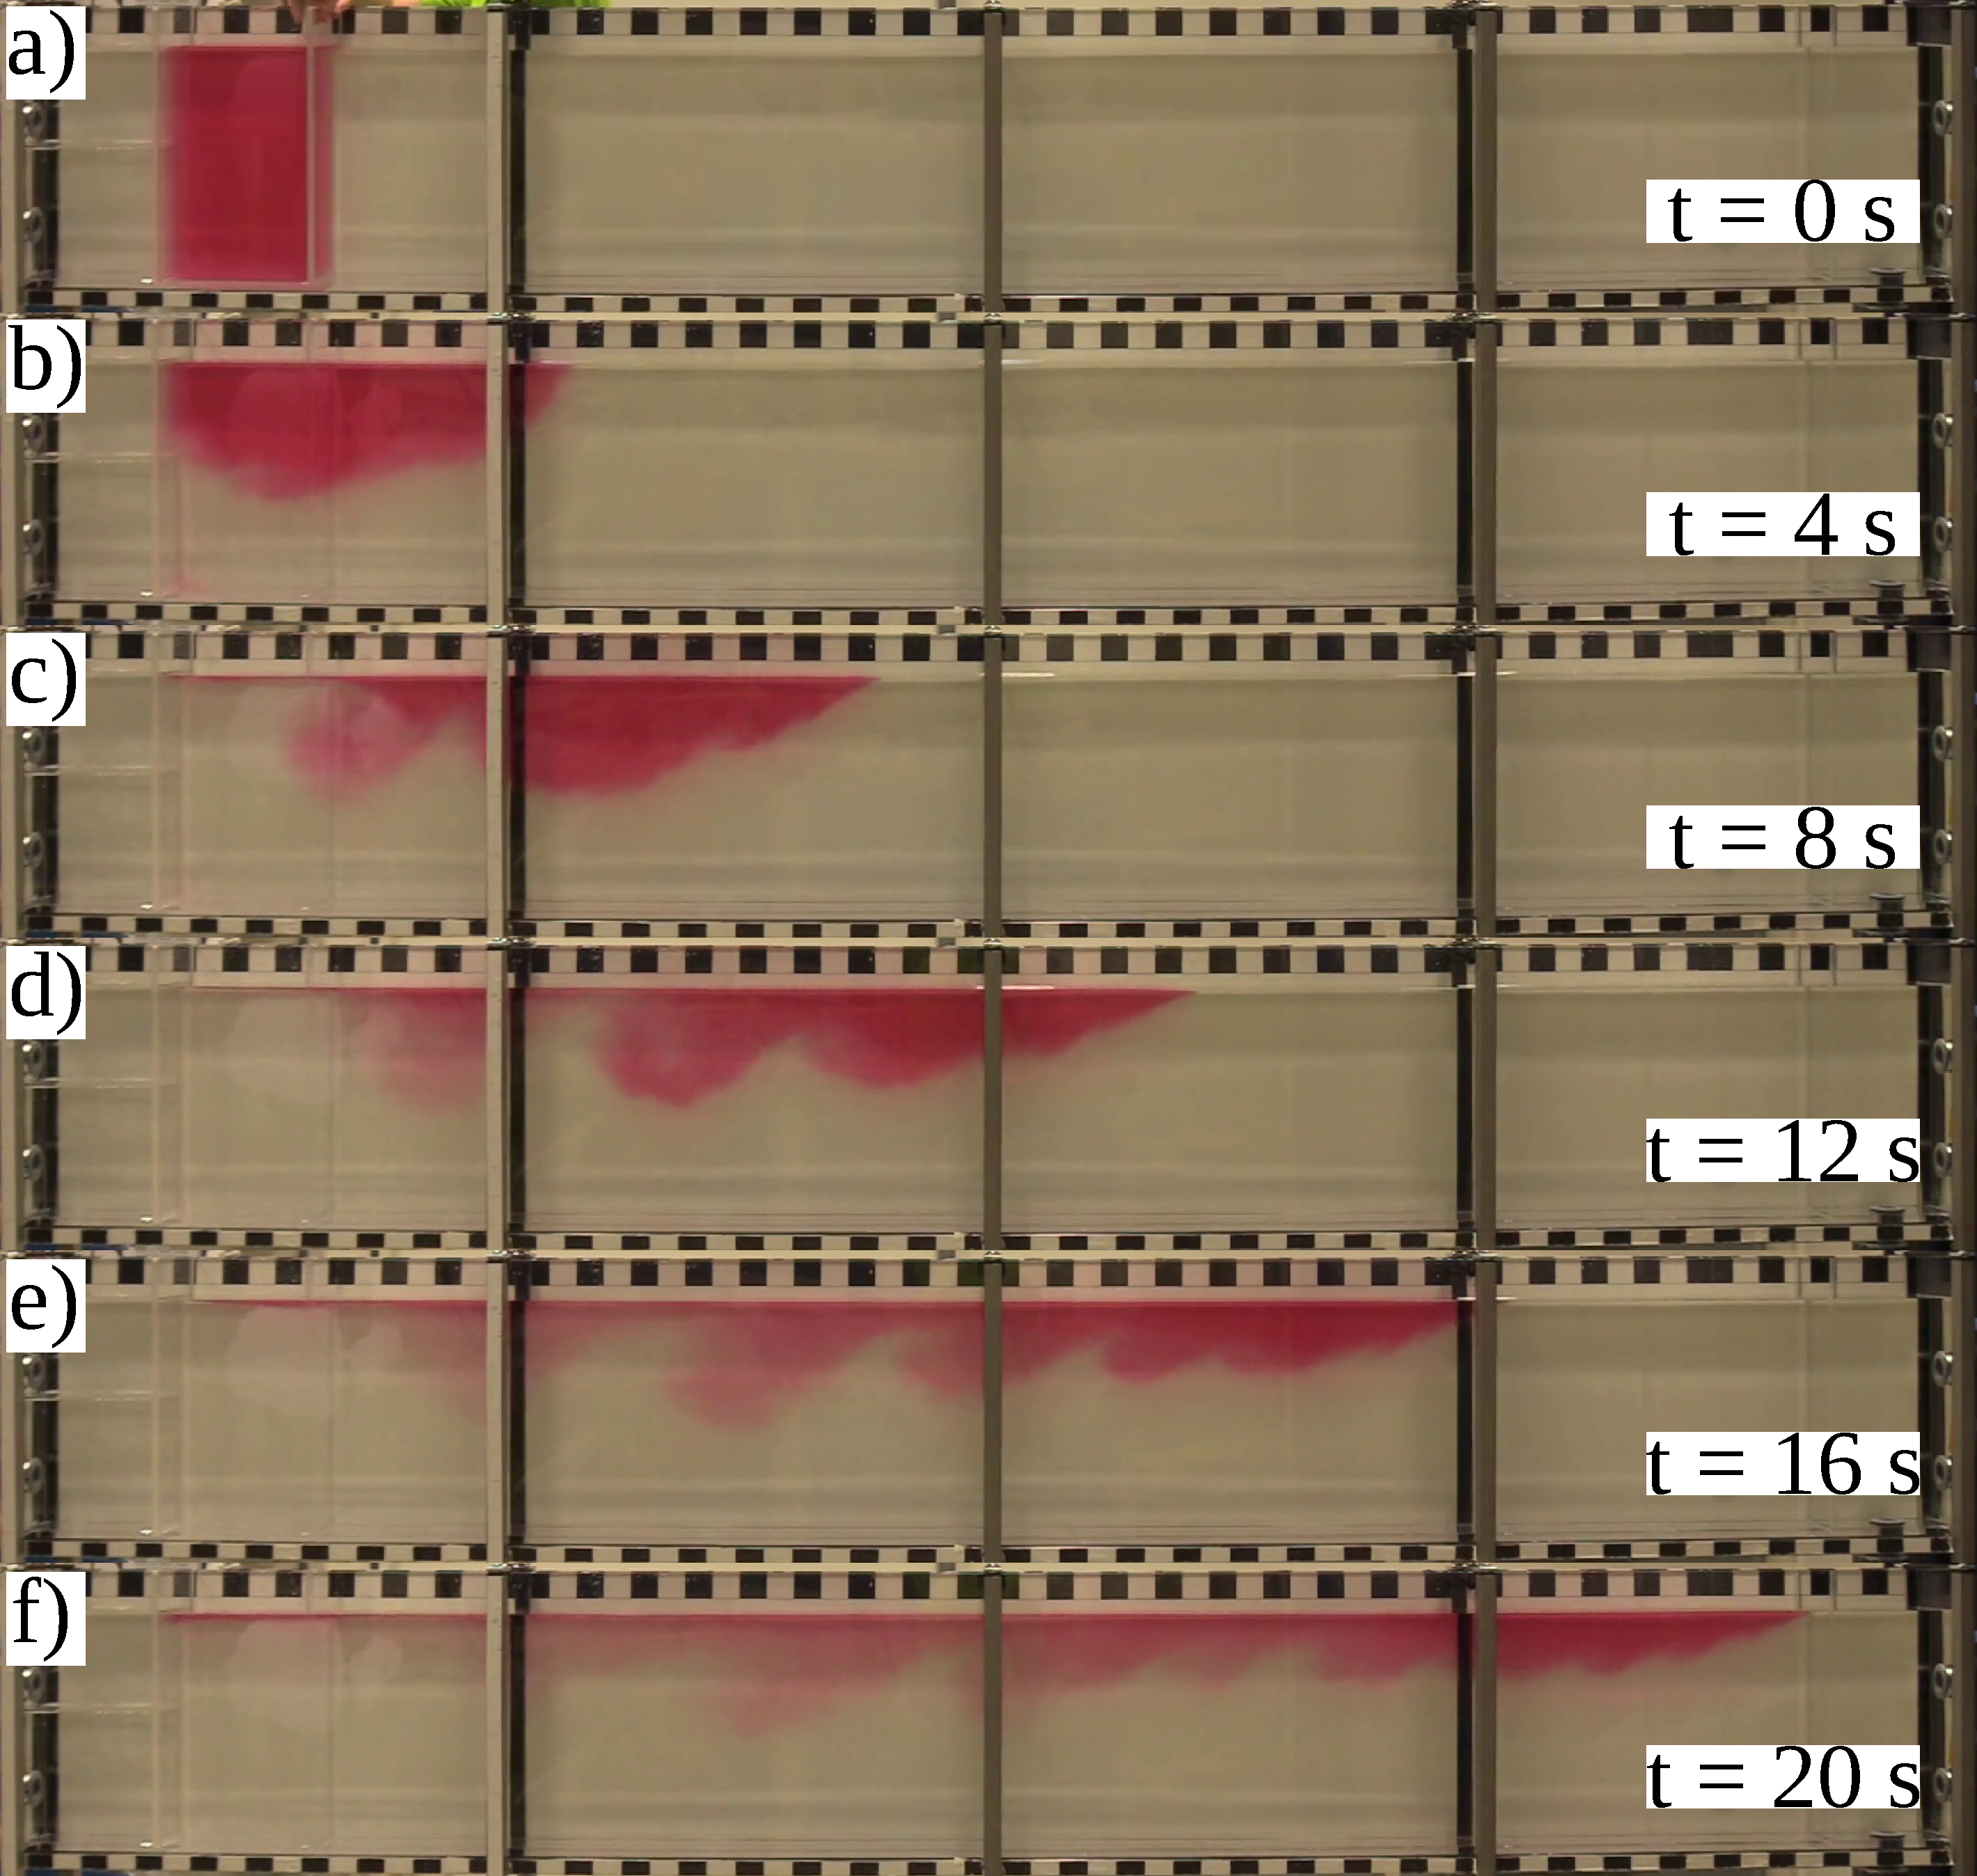
\includegraphics[width=0.9\textwidth]{GC9.pdf}}
  \caption{Sequence of images showing experiment GC9 ($\phi$ = 0, $g\prime$ = 0.563 m s$^{-2}$). }
  \label{fig:GC9}
\end{figure}

\subsection{Particle-bearing currents}
\label{subsec:res_w_parts}

Figure~\ref{fig:GC42} shows the evolution of the current in experiment GC42.

\begin{figure}[ht!]
  \centerline{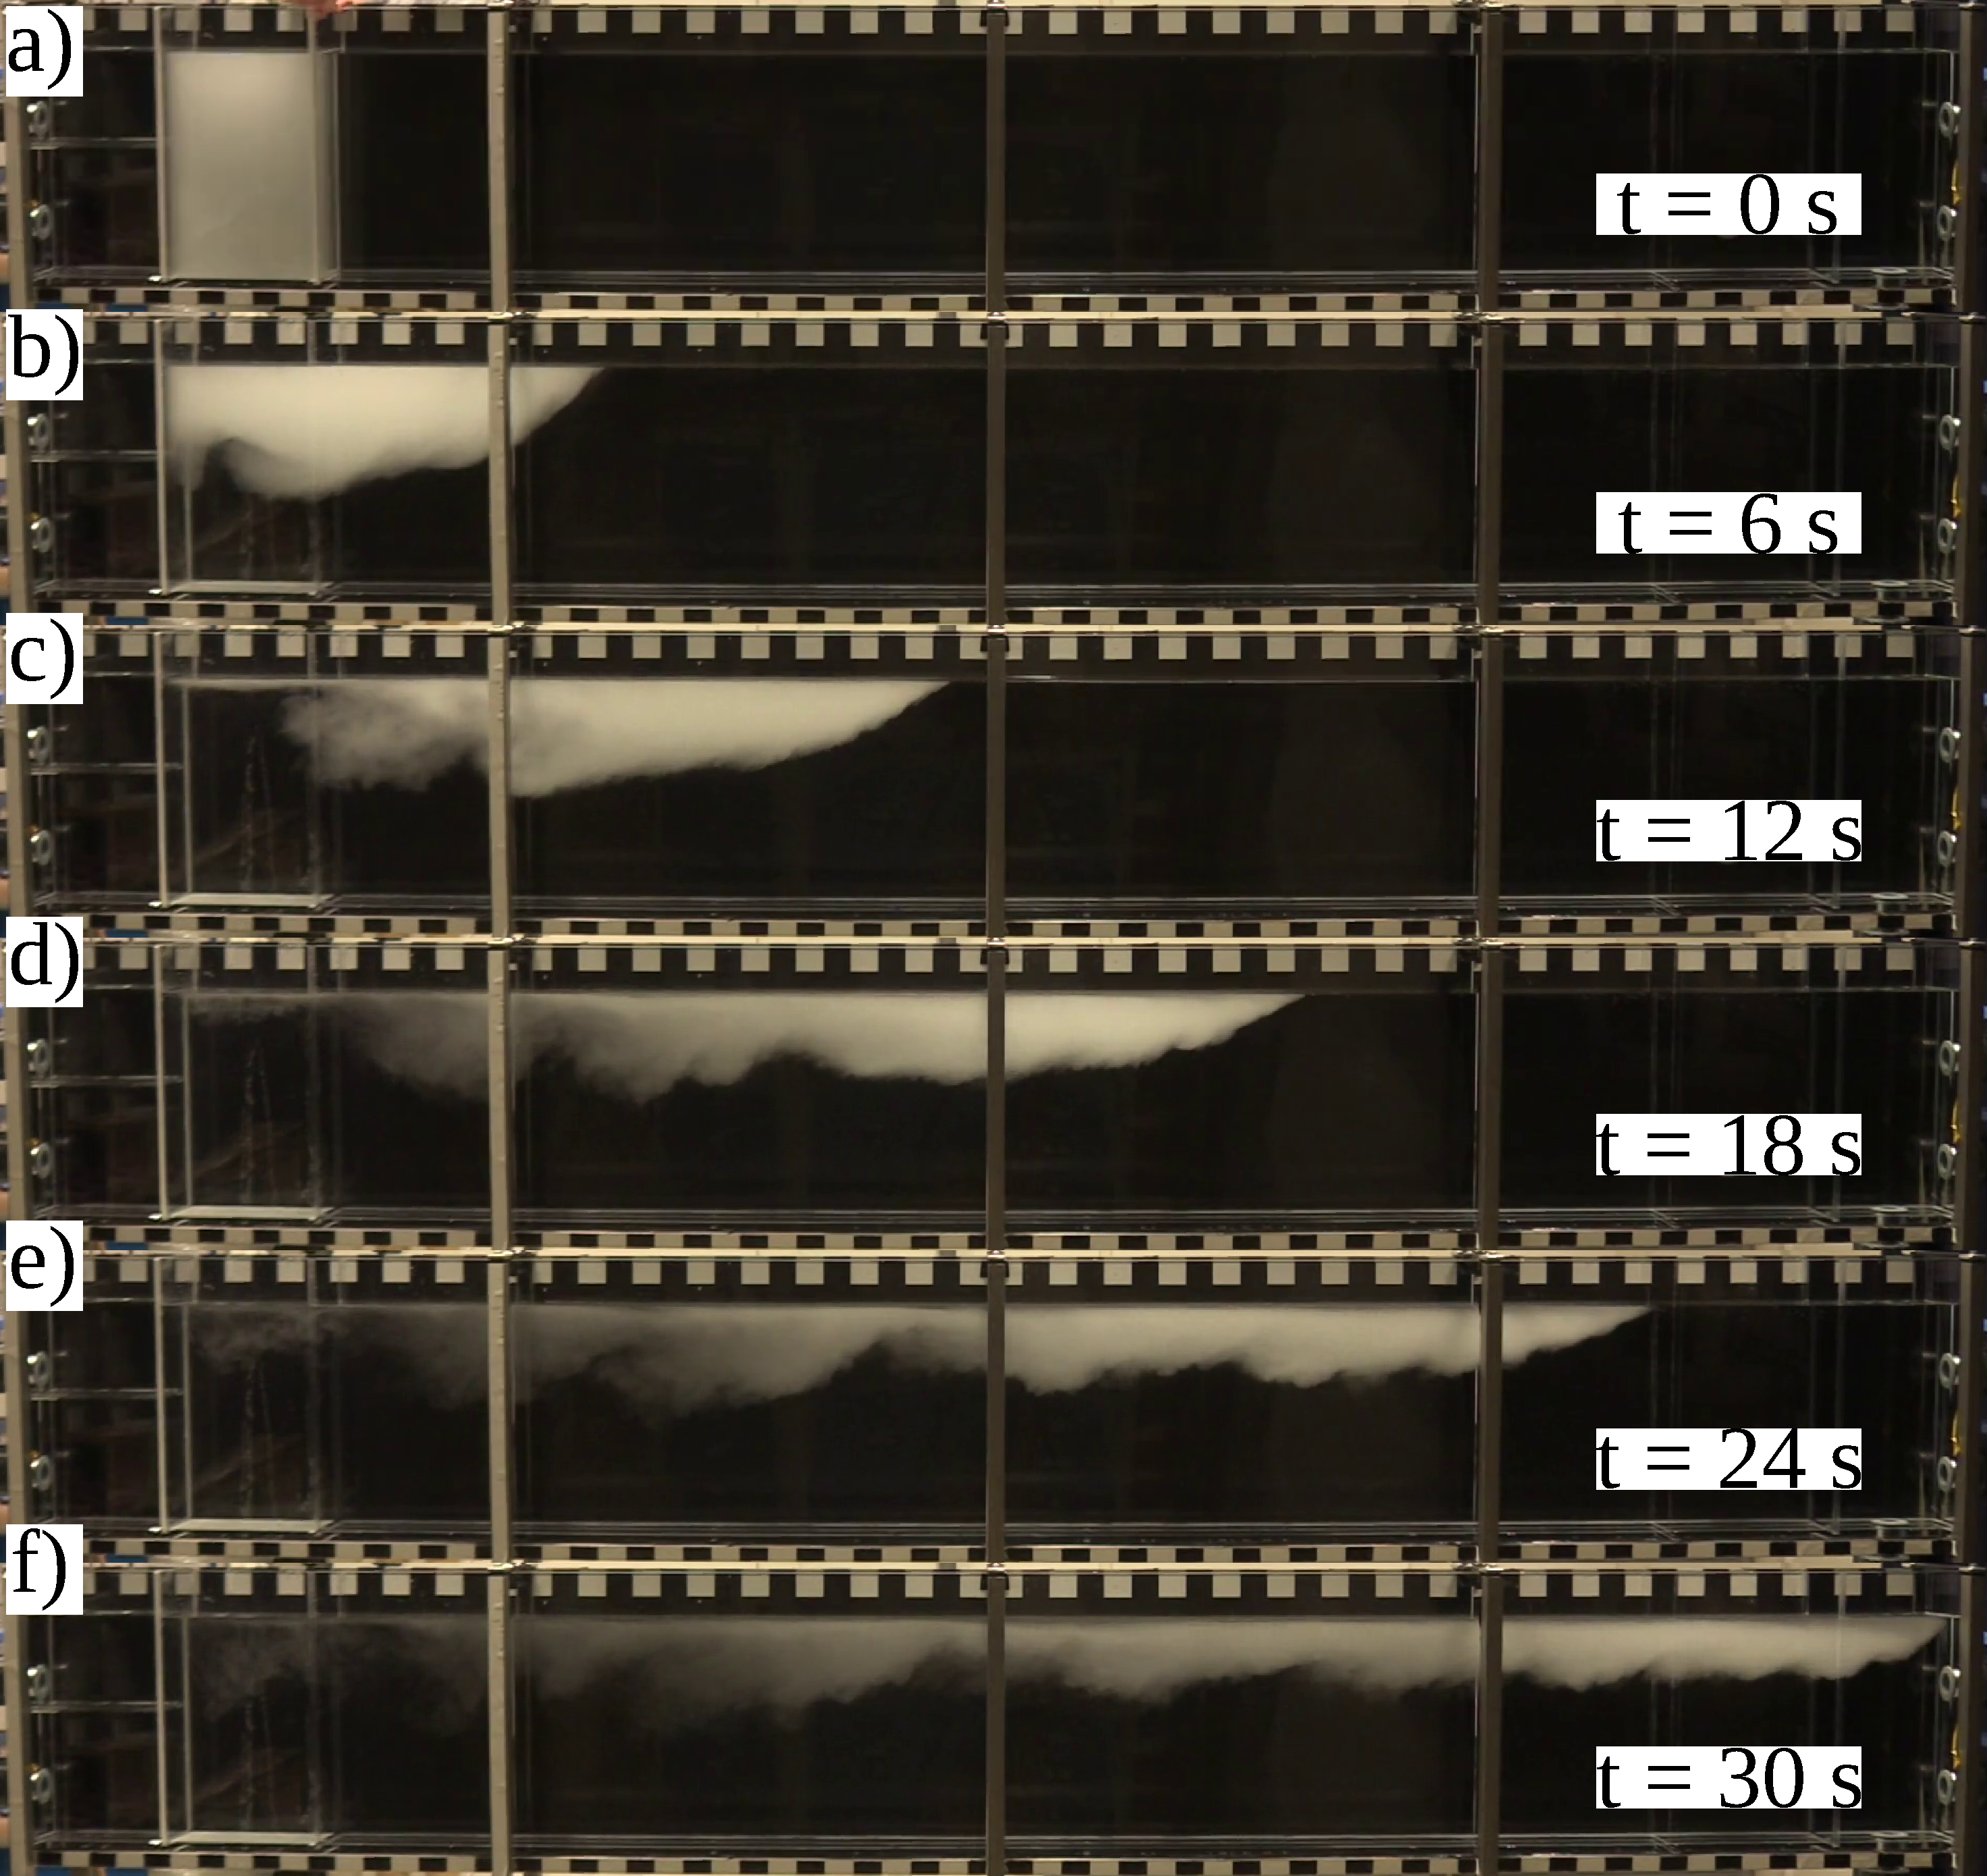
\includegraphics[width=0.9\textwidth]{GC42.pdf}}
  \caption{Sequence of images showing experiment GC42. }
  \label{fig:GC42}
\end{figure}
\section{Discussion}
\label{sec:dis}

\section{Conclusions}
\label{sec:conc}

\section*{Acknowledgements}
\label{sec:acknow}


%% The Appendices part is started with the command \appendix;
%% appendix sections are then done as normal sections
%% \appendix

%% \section{}
%% \label{}

%% If you have bibdatabase file and want bibtex to generate the
%% bibitems, please use
%%
%%  \bibliographystyle{elsarticle-harv} 
%%  \bibliography{<your bibdatabase>}

%% else use the following coding to input the bibitems directly in the
%% TeX file.

\begin{thebibliography}{00}

%% \bibitem[Author(year)]{label}
%% Text of bibliographic item

\bibitem[ ()]{}

\end{thebibliography}
\end{document}

\endinput
%%
%% End of file `elsarticle-template-harv.tex'.
